\documentclass[a4paper,12pt]{article}
\usepackage{amsmath}
\usepackage{amssymb}
\usepackage{graphicx}
\graphicspath{ {solution/} }
\begin{document}
\begin{center}
\textbf{{\Large Computer Vision}}\\
\textbf{{\Large Assignment 1}}\\
\end{center}
\textbf{Name:} Yash Sadhwani
\hspace*{70mm}
\textbf{NetID}: ys2913\\
\\ \\ \\
Note: For python version and packages installed kindly refer to master.py\\\\
\textbf{Solution 1: Image Filtering}\\ \\
\textbf{(a)}\\
$(X*F)[m,n]=\sum_{k,l}X[m-k,n-l].F[k,l]$\\ \\
\textbf{(a.1)}\\
For valid boundary condition, the kernel should not go outside the image matrix during convolution\\
$\therefore ,$ $m$ and $n$ start from 1(as $k,l \le$  1)\\ \\
$\Rightarrow(X*F)=
\begin{bmatrix}
za+by+dx+ew & zb+cy+ex+fw\\
zd+ey+gx+wh & ze+fy+hx+iw\\	
\end{bmatrix}
$\\
\\
\textbf{(a.2)}\\
Same boundary condition implies the output image size is same input image size\\
For the indexes in the first column and first row, the filter(F) goes outside the image dimensions, so we provide a zero padding to the image\\ \\
$\Rightarrow X = 
\begin{bmatrix}
0 & 0 & 0 & 0\\
0 & a & b & c\\
0 & d & e & f\\
0 & g & h & i\\
\end{bmatrix}\\ \\
$\\
$\Rightarrow (X*F)=
\begin{bmatrix}
aw & ax+bw & bx+cw\\
ay+dw & za+by+dx+ew & zb+cy+ex+fw\\
dy+gw & zd+ey+gx+wh & ze+fy+hx+iw\\
\end{bmatrix}
$\\
\\ \\
\textbf{(b)}\\
Row Size=$maxof(h-(maxof(0,i-1)),0)$\\
Column Size= $maxof(w-(maxof(0,j-1)),0)$\\
where $maxof(a,b)$, returns the maximum of the values of $a$ and $b$\\
\\ \\
\textbf{(c)}\\ \\
Input image:\\
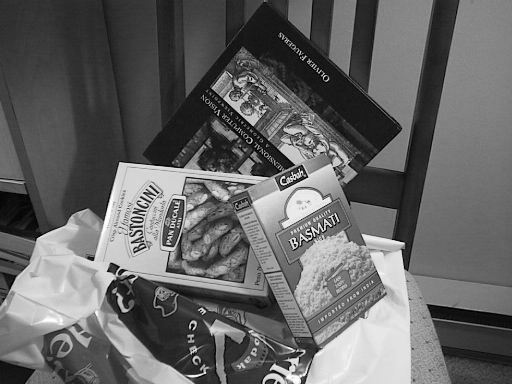
\includegraphics[width=10cm, height=8cm, angle=0]{scene.png}
\\ \\ \\
Blurred Image, Kernel Size = 3\\
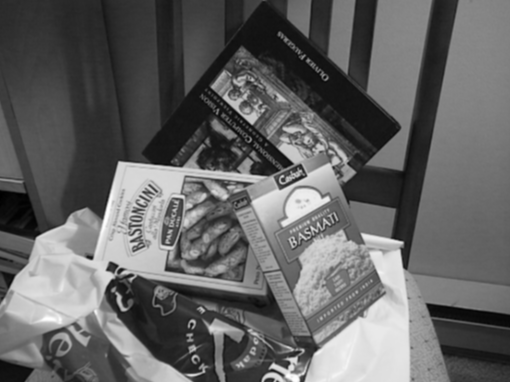
\includegraphics[width=10cm, height=8cm, angle=0]{ans_1_c_blurred_3.png}\\ \\ \\
\\ Blurred Image, Kernel Size = 5\\
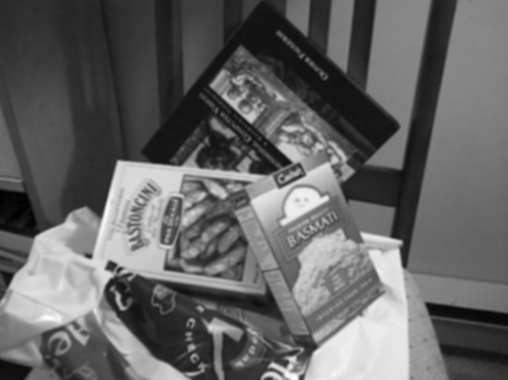
\includegraphics[width=10cm, height=8cm, angle=0]{ans_1_c_blurred_5.png}\\ \\ Blurred Image, Kernel Size = 7\\
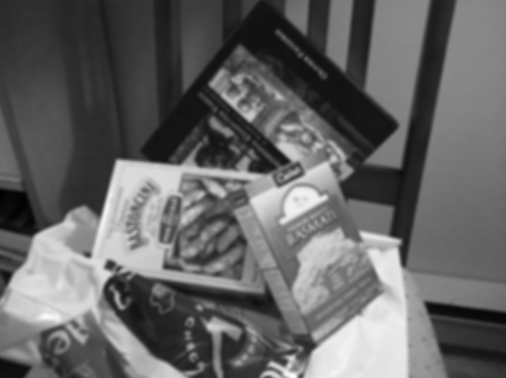
\includegraphics[width=10cm, height=8cm, angle=0]{ans_1_c_blurred_7.png}\\ \\
\\ \\ \\ \\ \\ 
\textbf{Solution 2: Image Alignment}\\ \\
Input Images:\\ \\
(a) Scene\\
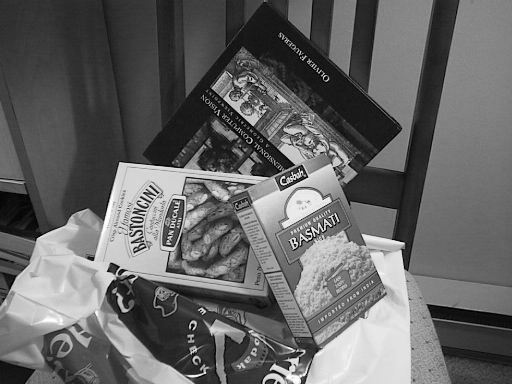
\includegraphics[width=10cm, height=8cm, angle=0]{scene.png}\\ \\
(a) Book\\
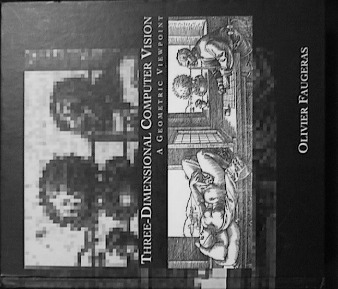
\includegraphics[width=10cm, height=8cm, angle=0]{book.png}\\ \\
\\
After SIFT detector, keypoints are:\\
(a) Scene\\
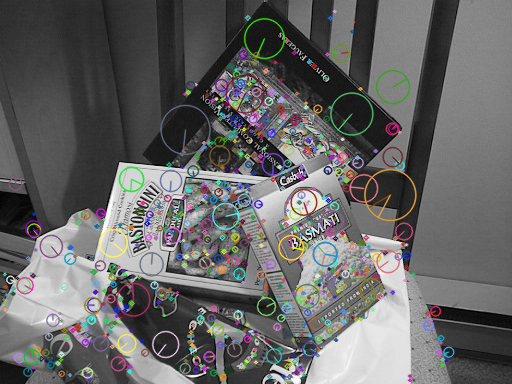
\includegraphics[width=10cm, height=8cm, angle=0]{ans_2_sift_scene.png}\\ \\
(a) Book\\
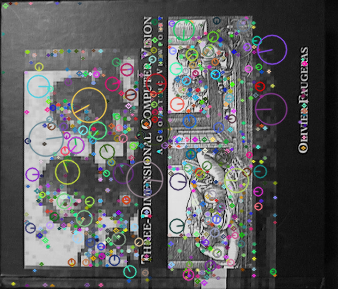
\includegraphics[width=10cm, height=8cm, angle=0]{ans_2_sift_book.png}\\ \\ \\ \\
\\ \\Good Feature matches before RANSAC(Lowe ratio = .9):\\
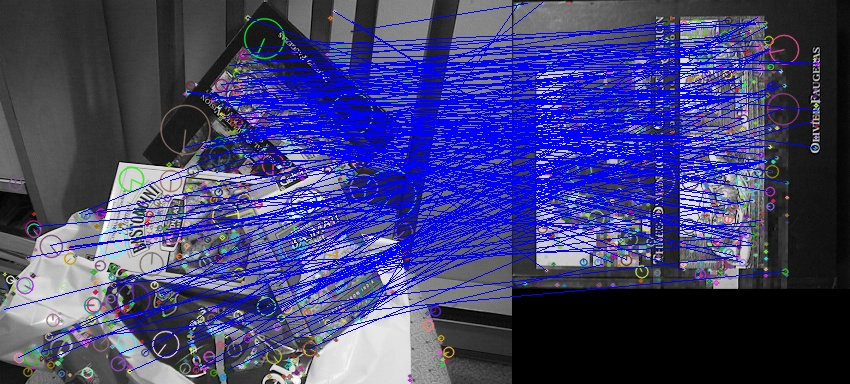
\includegraphics[width=17cm, height=8cm, angle=0]{ans_2_matches_before_RANSAC.jpg}\\ \\
\\ \\Inliers matches after RANSAC:\\
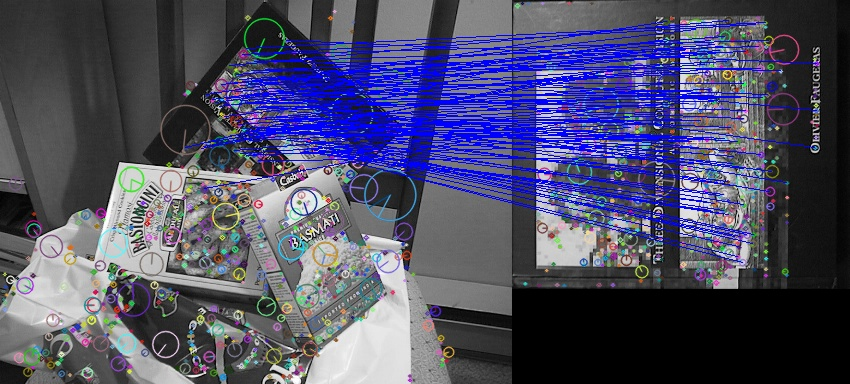
\includegraphics[width=17cm, height=8cm, angle=0]{ans_2_matches_after_RANSAC.jpg}\\ \\ \\ \\ \\
H Matrix after final refit:\\ \\
$\begin{bmatrix}
1.11134907 &  -1.20054516 &  37.95223962\\
1.21454692  &  1.07469998 & -330.28887393\\
\end{bmatrix}$\\ \\
Transformed image1(Scene):\\
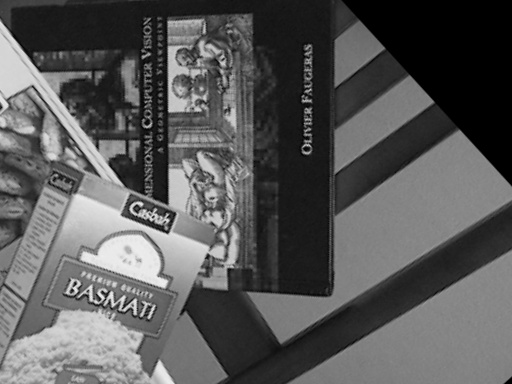
\includegraphics[width=10cm, height=8cm, angle=0]{ans_2_scene_transformed.jpg}\\ \\ \\ \\ \\
\\ \\ \\
\textbf{Solution 3: Estimating Camera Parameters}\\ \\
$P=
\begin{bmatrix}
1.27000127e-0 & 2.54000254e-01 & 3.81000381e-0 & 5.08000508e-0\\
5.08000508e-01 & 3.81000381e-01 &  2.54000254e-01 & 1.27000127e-01\\
1.27000127e-01 & -3.88578059e-16 & 1.27000127e-01 & 1.66533454e-16
\end{bmatrix}\\ \\ \\
C=
\begin{bmatrix}
1\\
-1\\
-1\\
\end{bmatrix}$(from method 1)
\\ \\
$C=
\begin{bmatrix}
1\\
-1\\
-1\\
\end{bmatrix}$(from alternate method)\\ \\
here C=(1,-1,-1) corresponding to the (x,y,z) coordinates\\
\\ \\ 
\textbf{Solution 3: Structure From Motion}\\ \\
$
M^1=
\begin{bmatrix}
-7.50914219 & 3.30837904 & -3.71763726\\
-4.53754376 & -1.57773527 & 7.74574759\\
\end{bmatrix}\\ \\
t^1=
\begin{bmatrix}
5.49560397189e-17 & -7.03141248929e-18\\
\end{bmatrix}
$\\ \\
First 10 World Coordinates=\\ \\
$
\begin{bmatrix}
0.0057716262048464534 & 0.064606281983366209 & -0.024976152508609184\\
0.00057609968845942949 & 0.068853630512852787 & -0.034581509689483474\\
-0.042935849081986173 & 0.063304789701081984 & 0.028617113082434285\\
0.047450383489819253 & 0.049042065349055641 & -0.012575472616125856\\
-0.04210186026210113 & 0.067892392631770784 & 0.011751637042499057\\
0.059619637747370967 & 0.046051799761544839 & -0.014383742867820666\\
0.0090916670806252976 & 0.060020489182699636 & -0.012299970374395277\\
0.010394894790726715 & 0.046020653847651458 & 0.035292747610496805\\
-0.025890805334956562 & 0.05702972054986117 & 0.033373747525897744\\
0.017455976600106268 & 0.040542636931378953 & 0.047318593420524906\\
\end{bmatrix}
$\\ \\
3D World points:\\
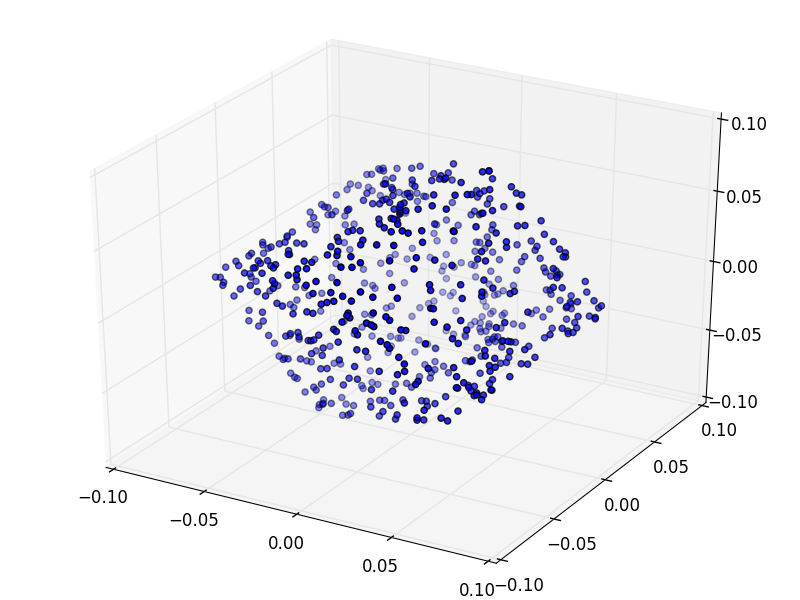
\includegraphics[width=10cm, height=8cm, angle=0]{ans_4_plot.png}\\
\end{document}